\documentclass[journal,comsoc]{IEEEtran}
\usepackage[T1]{fontenc}% optional T1 font encoding

\usepackage{ifpdf}
\usepackage{cite}
\ifCLASSINFOpdf
  \usepackage[pdftex]{graphicx}
\else
  \usepackage[dvips]{graphicx}
\fi
\usepackage{amsmath}
\interdisplaylinepenalty=2500
\usepackage[cmintegrals]{newtxmath}
\usepackage{bm}
\usepackage{algorithmic}
\usepackage{array}
\ifCLASSOPTIONcompsoc
  \usepackage[caption=false,font=normalsize,labelfont=sf,textfont=sf]{subfig}
\else
  \usepackage[caption=false,font=footnotesize]{subfig}
\fi
%\usepackage{fixltx2e}
%\usepackage{stfloats}
\ifCLASSOPTIONcaptionsoff
  \usepackage[nomarkers]{endfloat}
 \let\MYoriglatexcaption\caption
 \renewcommand{\caption}[2][\relax]{\MYoriglatexcaption[#2]{#2}}
\fi
\usepackage{url}
\usepackage{hyperref}
\usepackage{bbm}
% correct bad hyphenation here
\hyphenation{op-tical net-works semi-conduc-tor}


\begin{document}
\title{Spatial-Temporal Hand Pose Estimation For a Sequence of Depth Images}

\author{{Anonymous}% <-this % stops a space
\thanks{Anonymous}}

% The paper headers
\markboth{Journal of \LaTeX\ Class Files,~Vol.~14, No.~8, August~2015}%
{Shell \MakeLowercase{\textit{et al.}}: Bare Demo of IEEEtran.cls for IEEE Communications Society Journals}

% make the title area
\maketitle

\begin{abstract}
Abstract
\end{abstract}

% Note that keywords are not normally used for peerreview papers.
\begin{IEEEkeywords}
Hand pose estimation, Recurrent Network, Mixture of Experts.
\end{IEEEkeywords}


% For peer review papers, you can put extra information on the cover
% page as needed:
\ifCLASSOPTIONpeerreview
\begin{center} \bfseries EDICS Category: 3-BBND \end{center}
\fi
%
% For peerreview papers, this IEEEtran command inserts a page break and
% creates the second title. It will be ignored for other modes.
\IEEEpeerreviewmaketitle


\section{Introduction}\label{sec:introduction}
\IEEEPARstart{H}{and} pose estimation is an essential problem in computer vision, and plays an pivotal
role in vision application such as human-computer interface (HCI), augmentation reality (AR)~\cite{barsoum2016articulated}. So
far, there are a plenty of researches on this topic~\cite{guo2017region, quach2016depth, ge2017_3D,
wan2017crossing}, and major progresses have been made thanks to the improvement in deep learning
and low cost depth sensors. Nevertheless, hand is the most complex human part to analyse, and the
problem is still far from solved, it is still difficult to estimate hand pose in the practical scene
owing to several reasons. (1) the image quality is poor because of the commercial depth sensor, (2)
hand is a articulated object with high degrees of freedom (DoFs), the fingers are similar with each
other and apt to occlude each other, (3) in a real scenario, the application must process the depth
image real-timely, which increase the difficulty for estimation.

In general, the purpose of hand pose estimation is to estimate the 3D location of joints. Most existing
methods concentrate on the hand spatial structure modelling, such as the nodes in regression decision
forest and sparated stage in cascaded CNN, while ignoring the coherence between the current frame and
the previous frame. For instance, when we humans find the joint locations, we usually search in the
patches around the previous frame's joints. It reveals that the previous frame's pose provides abundant
information for pose estimation. However, many existing methods~\cite{oberweger2015hands, ge2017_3D} learn
the mapping from depth image or 3D voluetric representation to the hand pose. Some methods
~\cite{sun2015cascaded, ye2016spatial} explicitly model the hierarchical hand structure in addition. In
practice, depth images are in selected from videos, and video has time-varying dynamic properties.

\begin{figure}[t]
    \centering
    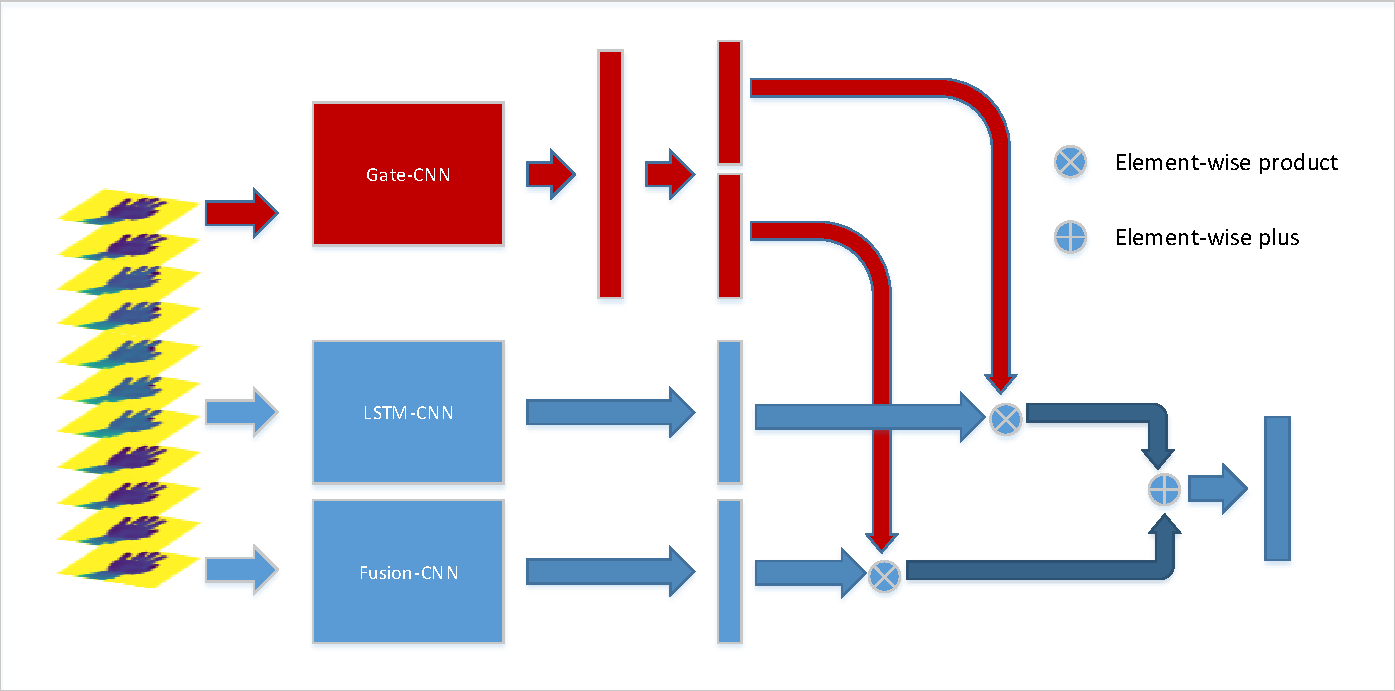
\includegraphics[width=1\linewidth]{src/network/architecture.pdf}
    \caption{The overview of architecture. The red branch is the \emph{Gate Network}, the blue
    branch is the expert networks. \emph{Temporal Network} extract the correlated features considering
    the sequentiality of input images and \emph{Spatial Network} employ the Deeply-fusion framework to
    fuse depth image and 3D volumetric representations, \emph{Gate Network} weights the prediction
    from each expert.}
\label{fig:architecture}
\end{figure}

Motivated by the observation above, we propose a method focus on the spatial structure as well as
temporal information. The different viewpoint for solving the problem is modelled as different part in
our method. Figure~\ref{fig:architecture} shows a holistic illustration for our approach. The first
part is denoted as \emph{Spatial Network} in this paper, which learns the mapping to hand pose from
spatial information. \emph{Spatial Network} works on a single depth image, with the depth image and
corresponding sliced 3D volumetric representation input into the network, spatial information extracted
hierarchically improve the performance of pose estimation. The second part is denoted as \emph{Temporal Network}.
The conventional works~\cite{tang2014latent, zhou2016model, tang2015opening} lay emphasis on the
hierarchical structure or spatial constraint of hand, while ignore the relationship
of the between frames. Motivated by this, we create this network pay attention to the time coherence property
in depth map video. The network take the previous features into account when estimating the pose in current frame,
in other words, the history is memorized by the network and affects the current prediction.

For the sake of accurately estimating the hand pose, we ensemble the aforementioned two networks as an
integration by Mixture of Experts~\cite{jacobs1991adaptive}. The networks for prediction task are called
\emph{experts}, and via \emph{gater} to outputs a set of weights, the final prediction is obtained by the
weighted combination of the experts outputs. By means of this ensemble approach, spatial information and temporal
coherence are thought to have in mind as a unified scheme. Moreover, the estimation network is evaluated on
two public datasets. Due to the practicability and efficiency, the network could run in in real-time on the GPU and achieve
the comparable or better results than state-of-art methods. We summary our contribution in the following two folds:
\begin{itemize}
  \item
  We integrate features from depth map and sliced 3D volumetric representation for hand pose
  estimation by deep fusion network. The experiment reveals that 3D volumetric representation
  benefits the hand pose estimation. Furthermore, we model the coherence among frames by LSTM,
  and implement a hand pose estimation system with an eye to accuracy, efficiency, robustness
  and stability simultaneously.
  \item
  Our proposed method could run about 75 fps on a single GPU, which meet the real-time demand
  in hand pose estimation. Moreover, we evaluate our approach on two public datasets (e.g. NYU
  and ICVL), and get the comparable or better results than state-of-art methods.
\end{itemize}

% needed in second column of first page if using \IEEEpubid
%\IEEEpubidadjcol

%-------------------------------------------------------------------------
\section{Related Work}\label{sec:related work}
\subsection{Hand Pose Estimation}
The approaches proposed in this area fall in three categories: data-driven, model-based and hybrid approaches.

Model-based approaches commonly evaluate the manually designed energy function on the basis of hand skeleton model,
the problem is formulated as an optimization problem that the objective function measure the discrepancy between
model hypothesis and the actual ones. Oikonomidis et.al ~\cite{oikonomidis2010markerless,oikonomidis2011efficient}
use Particle Swarm Optimization (PSO) solving the optimization problem about the hand model parameters.
With a discriminative initialization method, \cite{tagliasacchi2015robust} employ Iterative Closest Point (ICP)
for optimizing problem. \cite{qian2014realtime} use ICP-PSO for optimization and apply to a sphere-based hand motion model.
\cite{RoditakisMakrisArgyros2017} propose a method that explicitly considers constraints on the 3D locations of fingertips.
Different hand models are adopted in model based methods, such as surface model
~\cite{qian2014realtime,khamis2015learning} and gaussian model~\cite{sridhar2014real,tang2015opening},
etc. While the hand model is intuitive, these methods are sensitive to the initialization, and the errors are accumulated
during the estimation because of the temporal information used.

Data-driven approaches used in hand pose estimation are roughly divided into two camps: randomized decision forest (RDF)
and deep learning based methods. \cite{keskin2012hand,tang2013real,tang2014latent,sun2015cascaded,li20153d} employ RDF
for estimation. Specifically, \cite{keskin2012hand} use RDF-based method for hand part labelling and mean shift algorithm
as the joint finder. \cite{tang2013real} propose a semi-supervised transductive regression forest to label the realistic
dataset and the synthetic dataset, then refine joints by a data-driven, pseudo-kinematic technique. In \cite{tang2014latent},
a latent regression forest is learned for structured hand joints coarse-to-fine search, and \cite{li20153d} integrate
segmentation index points (SIP) achieving a better results. \cite{sun2015cascaded} hierarchically regress the joint
locations with a cascaded scheme. On the other side, CNN based methods learn the mapping from input to the hand pose,
comparing to the RDF based methods, a commonly better result could be achieved because the better features are learned.
Tompson et al.~\cite{tompson2014real} firstly employ CNN in hand pose estimation to regress the heat map and make use
of inverse kinematics algorithm as the post-processing. Oberweger et al.~\cite{oberweger2015hands} use segmented depth
map as input straightly regress 3D joint locations and do joint-specific refinement to increase the accuracy. Then in
~\cite{oberweger2015training}, a feedback loop framework is proposed, which is composed of a predictor for initialization,
a synthesizer for image generation and a updater for refinement. \cite{zhou2016model} design a network embedding the
forward kinematic process, which gets rid of the inconvenient post-processing. \cite{ye2016spatial} presents a method
by applying the kinematic hierarchy to both the input and feature space of the discriminative method and the optimization
of the generative method. Ge et al.~\cite{ge2016robust} predicts the heat-maps by a multi-view regression framework, and
\cite{ge2017_3D} improve this method by applying 3D CNN, which takes multi-view 3D volumetric representations as input for
regressing full 3D hand pose in a single pass. Wan et al.~\cite{wan2017crossing} use VAE and GAN to learn the manifold of
hand pose, with an alignment operation, pose space are projected into a corresponding depth map space via a shared latent
space.

Hybrid approaches\cite{keskin2013real, sharp2015accurate,madadi2017occlusion} retain the advantages of both data-driven and
model-based methods. \cite{keskin2013real} use the hand model for synthetic dataset generation followed by an RDF classifier,
then the mean-shift joint finder is adopted for final joint localization. \cite{sharp2015accurate} follows a different pipeline
which comprising hand RoI extraction, reinitialization and model fitting for hand tracking, hand model is used for extraction
and model fitting, the reinitialization step infer the distribution over hand poses via a layered discriminative model. In
\cite{madadi2017occlusion}, hand pose is recovered through a combination of part-based model fitting and data-driven approaches
in a single frame, and refine occluded joints in a sequence.

\subsection{LSTM}
introduce LSTM.

%------------------------------------------------------------------------
\section{Hand Pose Estimation}\label{sec:hand pose estimation}
In this section, we introduce our contributions to hand pose estimation.

\subsection{Problem Analysis}\label{sec:problem analysis}
% prepare the notation for problem
Our objective is to predict the hand joint locations in 3D space from a sequence of depth images,
the locations are represented as a set of keypoints. We denote a single depth image as $\mathit{I}$, and
the corresponding hand pose is
$\mathit{J}=\{\mathit{j}_i\}_i^K \in \mathbb{R}^{3 \times K}$ with $\mathit{j}_i=(x_i,y_i,z_i)$
represents the 3D position of $i$-th joint in the depth image $\mathit{I}$, $K$ is the number of joints,
it is different among datasets.

In this paper, we concentrate on the efficient 3D hand pose estimation from the depth images and
introduce a robust spatial-temporal hand pose estimation approach. In the natural scene, the camera
capture the consecutive frames and hand is contained in the frame.
The hand pose in the between frames is highly correlated. Inspired by the hand pose
tracking~\cite{quach2016depth}, we embed Long Short Time Memory (LSTM) into \emph{Temporal Network}
to extract features consider the sequentiality. Recurrent LSTM encode the original sequential
features into a correlated features for estimation. Furthermore, the spatial information of hand is
important, many approaches focus on tree structured skeleton of hand to address this problem (e.g.
~\cite{li20153d, wan2016direction, ye2016spatial}). And 3D volumetric representation could well reserve
the spatial information~\cite{deng2017hand3d} for solving pose estimation in 3D. We employ the
Deeply-fusion framework ~\cite{wang2016deeply} to fuse the features from depth image and sliced 3D
volumetric representations, which is called \emph{Spatial Network}. \emph{Temporal Network} and
\emph{Spatial Network} predict hand joint locations based on different features, which plays a
role of experts in the Mixture of Experts (MoE). In MoE, the different experts give out their
predictions and \emph{Gate Network} weights the predictions.

In this section, we introduce our method for hand pose estimation step by step.
The \emph{Temporal Network} and \emph{Spatial Network} we employed are discussed in Section
~\ref{sec:temporal netowork} and Section~\ref{sec:spatial network}, and \emph{Gate Network} is
discussed in Section~\ref{sec:gate network}.


% Figure ~\ref{fig:architecture} shows the entire architecture. Aspired by Mixture of Experts
% ~\cite{jacobs1991adaptive}, network is composed of two parts: \emph{Gate Network} and
% \emph{Expert Networks}, we use a \emph{Gate Network} to control two expert networks.
% Each expert predicts the 3D pose given the input image, the \emph{Gate Network} weights
% the prediction from each expert. The experts concentrate on different information.
% \emph{Temporal Network} takes temporal context into account between the consecutive frames.
% \emph{Spatial Network}, thinking over spatial information, fuses the features from depth
% map and 3D volumetric representation.

\subsection{Basic Network}\label{sec:basic network}
We first propose \emph{Basic Network} as the basic network for estimation. As shown in Figure
~\ref{fig:basic network}, the \emph{Basic Network} is a typical CNN architecture, which is composed
of several stacked convolution layers, with max-pooling layer do downsampling operation in between
them. The fully connected layers perform as a regressor for last regression. In addition, the activation
function used in network is ReLU, which provides non linear ability and improves the robustness. To resist
ooverfit, the Dropout is adopted in fully connected layers.

The \emph{Basic Network} performs a pre-trained network for \emph{Temporal Network}, and it could get a
satisfied result as shown in the experiments.

\subsection{Temporal Network}\label{sec:temporal netowork}
\begin{figure}[t]
    \centering
    \subfloat[Basic Netowrk]{
        \label{fig:basic network}
        \begin{minipage}[t]{116pt}
            \centering
            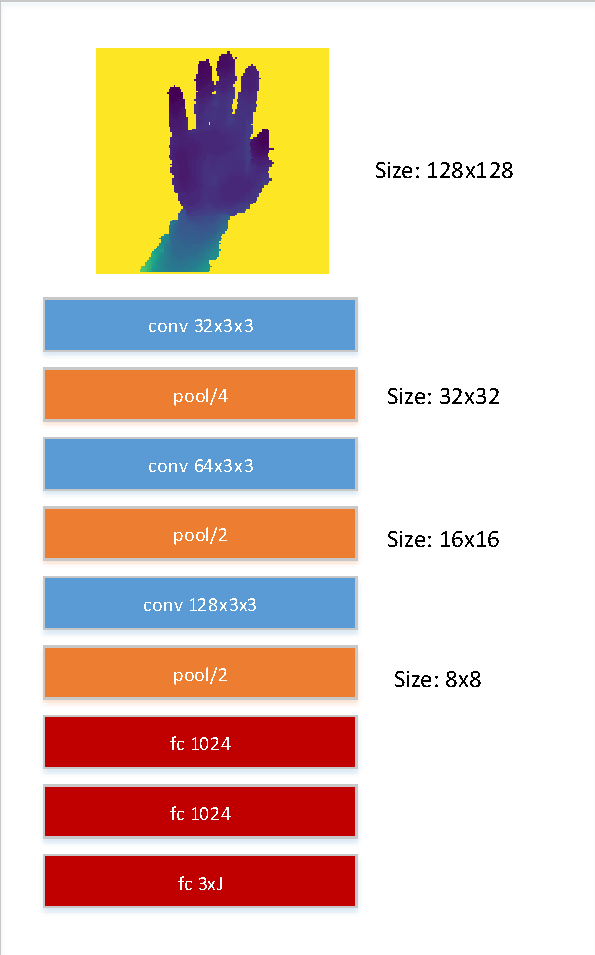
\includegraphics[width=1\linewidth]{src/network/baseline.pdf}
        \end{minipage}
    }
    \subfloat[Temporal Network]{
        \label{fig:temporal network}
        \begin{minipage}[t]{110pt}
            \includegraphics[width=1\linewidth]{src/network/temporal.pdf}
        \end{minipage}
    }
\caption{\emph{Basic Network} and \emph{Temporal Network}. In \emph{Basic Network}, convolution
layers and fully connected layers are followed by activation function is relu, and dropout is
adopted to resist overfit. In \emph{Temporal Network}, the parameters in previous layers are
borrowed from \emph{Basic Network}, lstm layer and last fully connected layer are trained when
the input is a sequence of images.}
\label{fig:basic and lstm network}
\end{figure}

As we know, the hand poses between successive frames are correlated (e.g. when grabbing, the joints
on fingers are most likely to be closer). Currently, an Recurrent Neural Network (RNN) with Long
Short-Term Memory (LSTM) units~\cite{zaremba2014learning} is widely used because they are expressive
and easy to train. The LSTM network is mostly used for modeling the long term temporal correspondence.
\cite{quach2016depth} use RNN regress the joint location straight forward, and training CNN and RNN
simultaneously. We do several modifications to extract robust features and have better result with
temporal information.

As is shown in Figure~\ref{fig:temporal network}, a sequence of frames $\{I_1, I_2, \dots, I_N\}$ is
taken as input and the network gives out the estimated pose. Think about the $t$-th depth image $I_t$,
the image flow through the convolution network and the feature extracted is denoted as follows,
\begin{equation}
\phi(I_t)=f_{\theta_c}(pre(I_t))
\end{equation}
where $f_{\theta_c}(\cdot)$ is a convolutional network with parameters $\theta_c$ and
$pre(\cdot)$ is the preprocessing to crop out the hand. The preprocessing step is declared
in Section.~\ref{sec:experiments}. The features are fed into LSTM and LSTM layer outputs its hidden
state,
\begin{equation}
h_t=f_{\theta_l}(h_{t-1}, \phi(I_t))
\end{equation}
where $f_{\theta_l}$ is the parameters in LSTM cell. The new features and original features
are concatenated then fed into the last fully connected layer and network give out the predictions.

In the training stage, the parameters of layers before lstm layer are borrowed from \emph{Basic Network}
and fixed, then we train LSTM and last fully connected layer solely.

\subsection{Spatial Network}\label{sec:spatial network}
According to the discussion in \cite{supancic2015depth, deng2017hand3d, ge2017_3D}, 3D
volumetric representation benefits the hand pose estimation. However, due to the high
cost of 3D convolution, the input is mostly small such as $32 \times 32 \times 32$ in
~\cite{deng2017hand3d, ge2017_3D}, it sacrifices the detail of depth image. We employ
an eclectic solution, the background is omitted in our 3D representation, and the space
is sliced into 8 pieces to preserve more details. The exemplar is shown in Figure
~\ref{fig:spatial network}.

The sliced 3D volumetric representation keeps the structure of hand, we can clearly find all
finger tips in the first layer, with a low cost for memory at the mean time. Nevertheless,
the depth information is deprecated in our sliced 3D volumetric representation, it makes harder
to estimate the hand joint locations. To obtain the hand structure and depth
information simultaneously, we input depth image and 3D volumetric representation at the
same time. In Figure~\ref{fig:spatial network}, we employ Deep-Fusion
framework~\cite{Chen_2017_CVPR} to fuse the features and the network is named as \emph{Spatial Network}.
The left part is same as \emph{Basic Network}, and the right part is similar with the left part.

In \emph{Spatial Network}, the different features are fused together hierarchically.
which could be expressed as:
\begin{equation}\label{eq:deep fusion}
\begin{aligned}
&f_0 = f_{depth} \oplus f_{3D} \\
&f_l = \mathbf{H}_l^{depth}(f_{l-1}) \oplus \mathbf{H}_l^{3D}(f_{l-1}) \\
&\forall l=1, \dots , L
\vspace{1em}
\end{aligned}
\end{equation}
The $\oplus$ is element-wise mean, $f_{depth}$ and $f_{3D}$ are the features output from
two pooling layers, $\mathbf{H}$ is the transformation for features,
$l$ is the index for layer.

Owing to the several fully connected layers, the network tends to overfitting, so we use
an auxiliary loss as the regularization as well as dropout. In Figure~\ref{fig:spatial network},
every fully connected layer is followed by a dropout layer, the nodes are dropout randomly
with 30\% probability. For the purpose of obtaining more representative capability for each input,
the auxiliary paths are added in training stage. As shown in the green boxes, the layers in the
auxiliary paths are same as the main network, the layers connected by the blue dotted line
share parameters. And in the training stage, the total losses are consist of three losses,
i.e. three regression loss in auxiliary paths and main network. When testing, the auxiliary
pathes are removed.
\begin{figure*}[t]
    \centering
    \includegraphics[width=0.5\linewidth]{src/network/spatial.pdf}
    \caption{\emph{Spatial Network}. Depth image and sliced 3D volumetric representation are input
    into \emph{Spatial Network}, the different features are fused together hierarchically. For the
    purpose of obtaining more representative capability for each input, the auxiliary paths are added
    in training stage, and the layers in the auxiliary paths are same as the main network. In the training
    stage, the total losses are consist of three losses, i.e. three regression loss in auxiliary paths
    and main network. When testing, the auxiliary pathes are removed.}
\label{fig:spatial network}
\end{figure*}

\subsection{Gate Network}\label{sec:gate network}
The foregoing \emph{Temporal Network} and \emph{Spatial Network} stand in the different views
for estimating the joints, we name the predictions as $\mathit{J}_{temp}$ and $\mathit{J}_{spa}$. To improve
the performance, we ensemble them via Mixture of Experts (MoE)~\cite{jacobs1991adaptive}, by adaptively integrating
different regressors for the last prediction.

\emph{Gate Network} weights two predictors, and give out the last prediction according to
the weights of predictions as follow:
\begin{equation}\label{eq:gate network}
\centering
\mathit{J}_{out} = \mathit{g}_1 \mathit{J}_{temp} + \mathit{g}_2 \mathit{J}_{spa}
\end{equation}
where $\mathit{g}_1$ and $\mathit{g}_2$ are the weight of \emph{Gate Network} and $\mathit{g}_1, \mathit{g}_2 \in
\mathbb{R}^{3 \times K}$. The final prediction $\mathit{J}_{out}$ is estimated as the weighted sum of each prediction.

Because \emph{Temporal Network} considers the temporal information and \emph{Spatial Network}
extracts the spatial information, mixture of experts infer the hand joint location based on
spatial and temporal features. Comparing with \emph{Basic Network}, \emph{Gate Network} outputs higher
dimension weights, so we employ a more complex network by increasing the number of convolution kernels.
Specifically, we double the parameters in \emph{Gate Network} than \emph{Basic Network}.

%-------------------------------------------------------------------------
\section{Experiments}\label{sec:experiments}
In this section, we evaluate our approach on two public datasets, NYU~\cite{tompson2014real}
and ICVL~\cite{tang2014latent}, for comparison with the state-of-art methods. In addition, we
do ablation experiments and analyse the performance of each component. We first describe our
experiment setting.

\subsection{Experiment Setting}\label{sec:experiment setting}
\subsubsection{Datasets}\label{sec:datasets}
NYU dataset is composed of 72K training and 8K testing images captured by PrimeSense. The
annotation is obtained by model-based tracking with a Particle Swarm Optimization processing.
This dataset is challenge because of its wider pose variation and noisy image as well as limited
annotation accuracy. ICVL dataset is smaller than NYU dataset, contains 22K frames for training
and 1.6K frames for testing. The resolution of images is only 320x240 and captured by Creative Interactive
Gesture Camera. The scale of image is small and the discrepancies between training and testing is
large, these makes the estimation hard. In the test sequences, the finger movement is more evident
than the train sequences.

\subsubsection{Evaluation Metrics}\label{sec:evaluation metrics}
The evaluation follows the standard metrics proposed in~\cite{oberweger2015hands}, including accuracy 
, pre-joint error distance and average error distance. As is mentioned above, we denote $j_{in}$ as 
the predicted $i$-th joint location in the $n$-th frame, $j_{in}^{gt}$ is the corresponding ground 
truth. The total number of frames is denoted as $N$, and $K$ is the number of joints in a frame. 

Per-joint error distance calculates the average Euclidean distance between the predicted 
joint location and the ground truth in 3D space.
\begin{equation}
err_i = \frac{\sum_n^N(\|j_{in} - j_{in}^{gt} \|)}{N}
\end{equation}

Average error distance computes the mean distance for all joints.
\begin{equation}
ave = \frac{\sum_i^K{err_i}}{K}
\end{equation}

Accuracy is the fraction of frames that all predicted joints from the ground truth in a 
frame below the given distance threshold $\delta$.
\begin{equation}
acc_{\delta} = \frac{\mathbbm{1}(max_i(\| j_{in} - j_{in}^{gt}\|) \leq \delta)}{N}
\end{equation}
where $\mathbbm{1}(*)$ is the indicator function equal to 1 only if $*$ is True.

Additionally, there are totally 36 annotated joints in NYU dataset, but we only
evaluate a subset of 14 joints for a fair comparison. In addition to ICVL dataset
, we evaluate total 16 annotated joints for comparison.

\subsubsection{Implementation Details}\label{sec:implementation}
We implement the training and testing with Caffe\cite{jia2014caffe}. The segmentation step
follows~\cite{oberweger2015hands} to extract a cube from the depth image, and the cube is
resized to a $128 \times 128$ depth image with the depth value normalized to [-1, 1]. Moreover, we
augment the dataset by random rotation.

The three components of network are trained separately. \emph{Basic Network} is pre-trained for
\emph{Temporal Network} with Adam, we set the learning rate as 1e-3
and train the network for 100,000 iterations, the learning rate is divided by 10 every 20,000
iterations and the mini-batch is set as 128. \emph{Spatial Network} is trained from scratch,
with the same setting as \emph{Basic Network}. \emph{Temporal Network} trained based on the \emph{Basic Network}
with the parameters fixed, and the configuration is same except that we only train the
network for 50,000 iterations.  To train the \emph{Gate Network}, the parameters are all fixed
but the parameters in gate branch and the network is trained for 50,000 iterations. Our training
takes place on machines equipped with a 12GB Titan X GPU and 64GB of RAM.

\subsection{Experiment Results}\label{sec:experiment results}
\subsubsection{Comparison with State-of-art}\label{sec:comparison}
We compare our approach with several state-of-art hand pose estimation methods~\cite{tompson2014real,oberweger2015hands, 
oberweger2015training, zhou2016model,tang2014latent,ge2017_3D,sinha2016deephand}. What is worth mention that some methods 
provide predicted joints but some not, we calculate the metrics of some methods~\cite{tompson2014real, oberweger2015hands,
oberweger2015training,zhou2016model,tang2014latent} available online and estimate the others from the figures in their paper. 
The average error distance of different methods is shown in Table~\ref{tab:mean error NYU} and Table~\ref{tab:mean error ICVL}.
% Table generated by Excel2LaTeX from sheet 'comparisonNYU'
\begin{table}[htbp]
  \centering
  \caption{Comparison of different methods on NYU dataset.}
    \begin{tabular}{|l|c|}
    \hline
    Methods & \multicolumn{1}{l}{Average joint error (mm)} \\
    \hline
    HeatMap~\cite{tompson2014real} & 21.02 \\
    DeepPrior~\cite{oberweger2015hands} & 19.73 \\
    Feedback~\cite{oberweger2015training} & 15.97 \\
    DeepModel~\cite{zhou2016model} & 16.90 \\
    Lie-X~\cite{xu2017lie} & 14.51 \\
    Ours  & 14.83 \\
    \hline
    \end{tabular}%
  \label{tab:mean error NYU}%
\end{table}%

% Table generated by Excel2LaTeX from sheet 'average joint error'
\begin{table}[htbp]
  \centering
  \caption{Comparison of different methods on ICVL dataset.}
    \begin{tabular}{|l|r|}\hline
    Methods & \multicolumn{1}{l}{Average joint error (mm)} \\\hline
    LRF~\cite{tang2014latent}   &  0\\
    DeepPrior~\cite{oberweger2015hands} &  0\\
    DeepModel~\cite{zhou2016model} &  0\\
    Ours  &  0\\
    \hline
    \end{tabular}%
  \label{tab:mean error ICVL}%
\end{table}%
\paragraph{NYU Dataset}\label{sec:nyu dataset}
We compare our method with several approaches on NYU dataset, including 3DCNN~\cite{ge2017_3D}, DeepModel~\cite{zhou2016model}, 
Feedback~\cite{oberweger2015training}, DeepPrior~\cite{oberweger2015hands}, Matrix~\cite{sinha2016deephand}, HeatMap~\cite{tompson2014real}, 
Lie-X~\cite{xu2017lie}. The accuracy and the pre-joint error distance are shown in Figure~\ref{fig:comparison NYU}. The result reveals 
that our proposed method has a comparable performance with state-of-art methods. Our method outperform most methods except 3DCNN and Lie-X. 
Comparing with 3DCNN, our method is better around 9-12mm and 60-80mm. Lie-X stands out over the range of 20-48mm, but our method overtakes 
at other times. 


\begin{figure*}[t]\footnotesize
\centering
    \subfloat[]{
        \label{fig:comparison NYU}
        \begin{minipage}[t]{200pt}
            \centering
            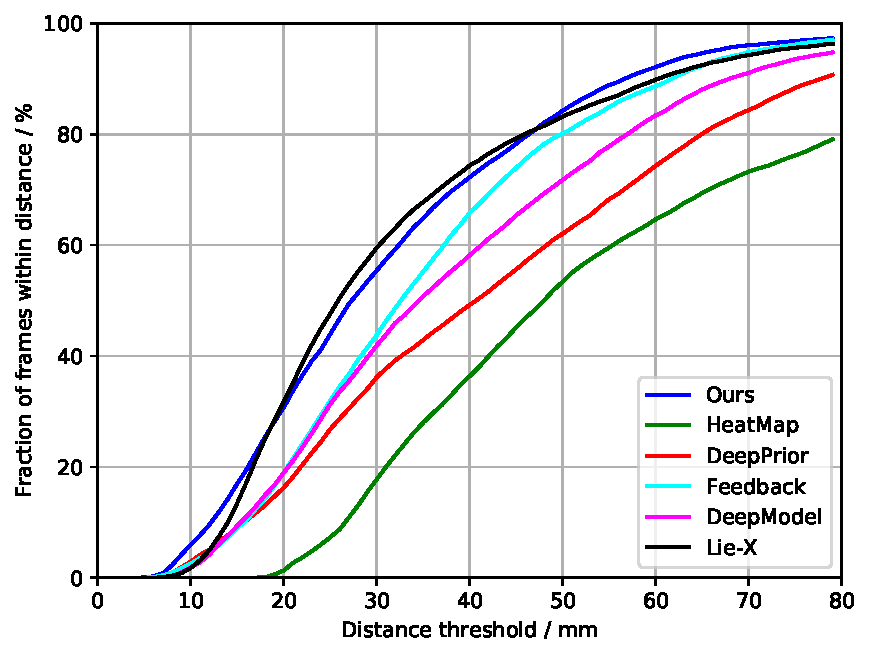
\includegraphics[width=1\linewidth]{src/experiment/eval/NYU_comparison/comparison_frameswithin.pdf}
        \end{minipage}
    }
    \subfloat[]{
        \label{fig:joint mean NYU}
        \begin{minipage}[t]{260pt}
            \centering
            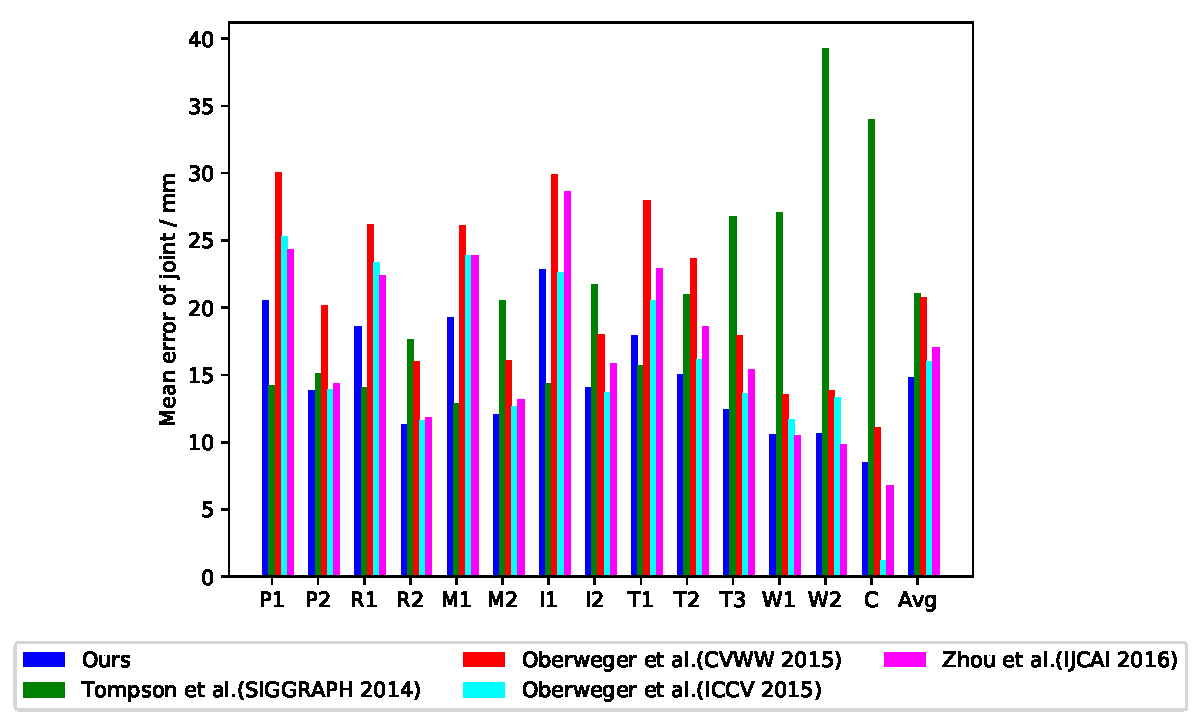
\includegraphics[width=1\linewidth]{src/experiment/eval/NYU_comparison/comparison_joint_mean.pdf}
        \end{minipage}
    }
    \caption{Qualitative results for NYU dataset.}
    \label{fig:Qualitative result NYU}
\end{figure*}

\paragraph{ICVL Dataset}\label{sec:icvl dataset}
On ICVL dataset, we compare our proposed method against three approaches~\cite{tang2014latent,oberweger2015hands,zhou2016model}.
\subsubsection{Ablation}\label{sec:ablation}
To show the effects of different parts in mixed network, we do the ablation experiments. We
show the test result on NYU and ICVL dataset in Figure~\ref{fig:Qualitative result ablation}.

\begin{figure*}[t]\footnotesize
\centering
    \subfloat[]{
        \label{fig:ablation NYU}
        \begin{minipage}[t]{200pt}
            \centering
            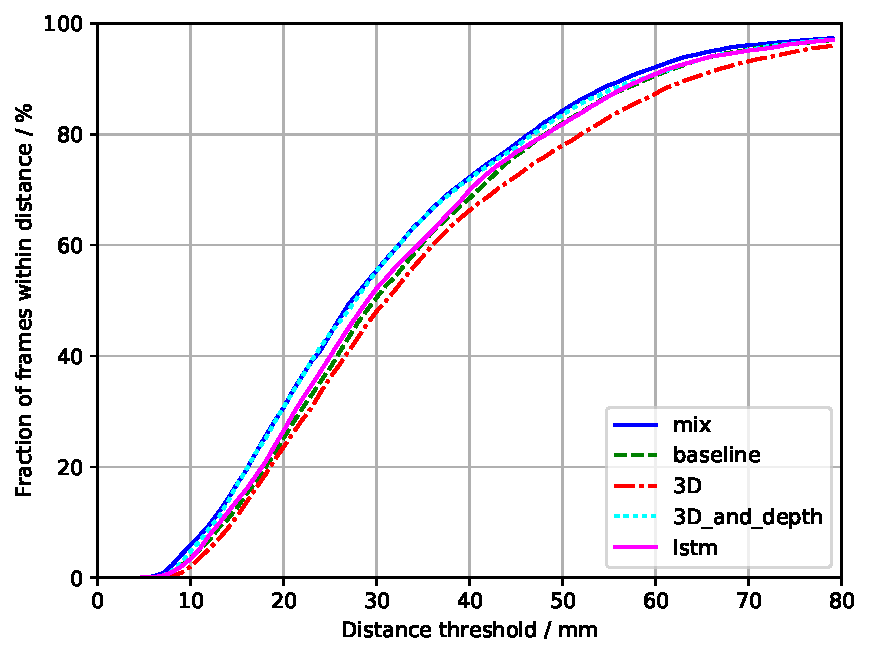
\includegraphics[width=1\linewidth]{src/experiment/eval/NYU_ablation/ablation_frameswithin.pdf}
        \end{minipage}
    }
    \subfloat[]{
        \label{fig:ablation joint mean NYU}
        \begin{minipage}[t]{180pt}
            \centering
            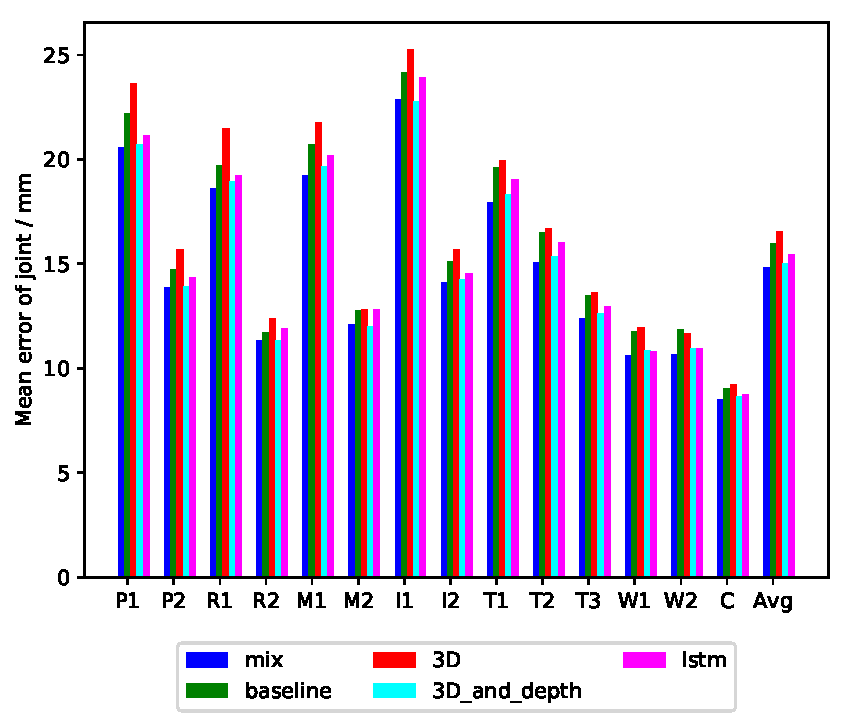
\includegraphics[width=1\linewidth]{src/experiment/eval/NYU_ablation/ablation_joint_mean.pdf}
        \end{minipage}
    }
    \caption{Qualitative results for ablation experiments.}
    \label{fig:Qualitative result ablation}
\end{figure*}

\section{Conclusion}\label{sec:conclusion}
The conclusion goes here.

% An example of a floating figure using the graphicx package.
% Note that \label must occur AFTER (or within) \caption.
% For figures, \caption should occur after the \includegraphics.
% Note that IEEEtran v1.7 and later has special internal code that
% is designed to preserve the operation of \label within \caption
% even when the captionsoff option is in effect. However, because
% of issues like this, it may be the safest practice to put all your
% \label just after \caption rather than within \caption{}.
%
% Reminder: the "draftcls" or "draftclsnofoot", not "draft", class
% option should be used if it is desired that the figures are to be
% displayed while in draft mode.
%
%\begin{figure}[!t]
%\centering
%\includegraphics[width=2.5in]{myfigure}
% where an .eps filename suffix will be assumed under latex,
% and a .pdf suffix will be assumed for pdflatex; or what has been declared
% via \DeclareGraphicsExtensions.
%\caption{Simulation results for the network.}
%\label{fig_sim}
%\end{figure}

% Note that the IEEE typically puts floats only at the top, even when this
% results in a large percentage of a column being occupied by floats.


% An example of a double column floating figure using two subfigures.
% (The subfig.sty package must be loaded for this to work.)
% The subfigure \label commands are set within each subfloat command,
% and the \label for the overall figure must come after \caption.
% \hfil is used as a separator to get equal spacing.
% Watch out that the combined width of all the subfigures on a
% line do not exceed the text width or a line break will occur.
%
%\begin{figure*}[!t]
%\centering
%\subfloat[Case I]{\includegraphics[width=2.5in]{box}%
%\label{fig_first_case}}
%\hfil
%\subfloat[Case II]{\includegraphics[width=2.5in]{box}%
%\label{fig_second_case}}
%\caption{Simulation results for the network.}
%\label{fig_sim}
%\end{figure*}
%
% Note that often IEEE papers with subfigures do not employ subfigure
% captions (using the optional argument to \subfloat[]), but instead will
% reference/describe all of them (a), (b), etc., within the main caption.
% Be aware that for subfig.sty to generate the (a), (b), etc., subfigure
% labels, the optional argument to \subfloat must be present. If a
% subcaption is not desired, just leave its contents blank,
% e.g., \subfloat[].


% An example of a floating table. Note that, for IEEE style tables, the
% \caption command should come BEFORE the table and, given that table
% captions serve much like titles, are usually capitalized except for words
% such as a, an, and, as, at, but, by, for, in, nor, of, on, or, the, to
% and up, which are usually not capitalized unless they are the first or
% last word of the caption. Table text will default to \footnotesize as
% the IEEE normally uses this smaller font for tables.
% The \label must come after \caption as always.
%
%\begin{table}[!t]
%% increase table row spacing, adjust to taste
%\renewcommand{\arraystretch}{1.3}
% if using array.sty, it might be a good idea to tweak the value of
% \extrarowheight as needed to properly center the text within the cells
%\caption{An Example of a Table}
%\label{table_example}
%\centering
%% Some packages, such as MDW tools, offer better commands for making tables
%% than the plain LaTeX2e tabular which is used here.
%\begin{tabular}{|c||c|}
%\hline
%One & Two\\
%\hline
%Three & Four\\
%\hline
%\end{tabular}
%\end{table}


% Note that the IEEE does not put floats in the very first column
% - or typically anywhere on the first page for that matter. Also,
% in-text middle ("here") positioning is typically not used, but it
% is allowed and encouraged for Computer Society conferences (but
% not Computer Society journals). Most IEEE journals/conferences use
% top floats exclusively.
% Note that, LaTeX2e, unlike IEEE journals/conferences, places
% footnotes above bottom floats. This can be corrected via the
% \fnbelowfloat command of the stfloats package.

% if have a single appendix:
%\appendix[Proof of the Zonklar Equations]
% or
%\appendix  % for no appendix heading
% do not use \section anymore after \appendix, only \section*
% is possibly needed

% use appendices with more than one appendix
% then use \section to start each appendix
% you must declare a \section before using any
% \subsection or using \label (\appendices by itself
% starts a section numbered zero.)
%


\appendices
\section{Gate Network Architecture}\label{sec:gate network architecture}
Appendix one text goes here.


% use section* for acknowledgment
\section*{Acknowledgment}


The persons would like to thank...


% Can use something like this to put references on a page
% by themselves when using endfloat and the captionsoff option.
\ifCLASSOPTIONcaptionsoff
  \newpage
\fi



% trigger a \newpage just before the given reference
% number - used to balance the columns on the last page
% adjust value as needed - may need to be readjusted if
% the document is modified later
%\IEEEtriggeratref{8}
% The "triggered" command can be changed if desired:
%\IEEEtriggercmd{\enlargethispage{-5in}}

% references section

% can use a bibliography generated by BibTeX as a .bbl file
% BibTeX documentation can be easily obtained at:
% http://mirror.ctan.org/biblio/bibtex/contrib/doc/
% The IEEEtran BibTeX style support page is at:
% http://www.michaelshell.org/tex/ieeetran/bibtex/
%\bibliographystyle{IEEEtran}
% argument is your BibTeX string definitions and bibliography database(s)
%\bibliography{IEEEabrv,../bib/paper}
%
% <OR> manually copy in the resultant .bbl file
% set second argument of \begin to the number of references
% (used to reserve space for the reference number labels box)
\bibliography{wu}
\bibliographystyle{IEEEtran}

% biography section
%
% If you have an EPS/PDF photo (graphicx package needed) extra braces are
% needed around the contents of the optional argument to biography to prevent
% the LaTeX parser from getting confused when it sees the complicated
% \includegraphics command within an optional argument. (You could create
% your own custom macro containing the \includegraphics command to make things
% simpler here.)
%\begin{IEEEbiography}[{\includegraphics[width=1in,height=1.25in,clip,keepaspectratio]{mshell}}]{Michael Shell}
% or if you just want to reserve a space for a photo:

% insert where needed to balance the two columns on the last page with
% biographies
%\newpage

%\begin{IEEEbiographynophoto}{Jane Doe}
%Biography text here.
%\end{IEEEbiographynophoto}

% You can push biographies down or up by placing
% a \vfill before or after them. The appropriate
% use of \vfill depends on what kind of text is
% on the last page and whether or not the columns
% are being equalized.

%\vfill

% Can be used to pull up biographies so that the bottom of the last one
% is flush with the other column.
%\enlargethispage{-5in}



% that's all folks
\end{document}


